\documentclass[10pt,a4paper]{article}
\usepackage[margin=2.2cm]{geometry}
\usepackage[T1]{fontenc}
\usepackage{lmodern}
\usepackage{amsmath,amssymb,bm,booktabs,graphicx,array}
\usepackage{xcolor}
\usepackage{microtype}
\usepackage{hyperref}
\hypersetup{colorlinks=true,linkcolor=blue!45!black,urlcolor=blue!45!black,citecolor=blue!45!black}
\makeatletter
\let\tableinput\@@input
\makeatother
\newcommand{\vect}[1]{\bm{#1}}
\newcommand{\R}{\mathbb{R}}
\newcommand{\RMSE}{\operatorname{RMSE}}
\newcommand{\clip}{\operatorname{clip}}
\newcommand{\sigmoid}{\operatorname{sigmoid}}
\setlength{\parskip}{4pt}
\setlength{\parindent}{0pt}
\setlength{\emergencystretch}{2em}
\title{Asteroid lightcurve inversion\\\large Methods and reconstruction results}
\author{HAC--DTU project}
\date{}

\begin{document}
\maketitle
\begin{abstract}
We reconstruct non-convex asteroid surfaces from multi-view rotational
lightcurves using a spherical-harmonic octantoid mesh, differentiable image
formation, empirical acquisition calibration, and a regularized staged Adam
solver. We specify the forward model and optimization procedure, compare
harmonic representations, and report saved degree-4 fits from a ten-asteroid
experiment. Mesh and image comparisons expose the distinction between
photometric agreement and geometric fidelity. Public references permit
geometry evaluation for asteroids 1--3; interpretations of asteroids 4--10
are conditional on transferred calibration. All photometric errors are
root-mean-square errors (RMSE) of normalized intensity lightcurves.
\end{abstract}

\section{Problem, observations, and scope}
For asteroid $A$, the simulated dataset contains $N=360$ rotation samples
and $C=21$ independent cameras. Seven camera azimuths each provide
horizontal, upper, and lower views. The duplicated horizontal channel is
removed only after checking equality; the separate real-data loader can
retain 28 channels. Public reference surfaces exist for asteroids 1--3;
the shapes of asteroids 4--10 are hidden.

Let $\vect p\in\R^P$ be shape coefficients, $F$ fixed triangle connectivity,
and $\vartheta$ fixed acquisition parameters. The forward map is
\begin{equation}
 \vect p\ \longmapsto\ (\vect v_i(\vect p),F)
 \ \longmapsto\ I_{tj,u}(\vect p;\vartheta)
 \ \longmapsto\ B_{tj}\ \longmapsto\ \widehat y_{tj},
 \label{eq:pipeline}
\end{equation}
where $t$, $j$, and $u$ index rotation, camera, and image pixel.
Only the shape coefficients are fitted. The rotation axis is the world
$z$ axis; rotation samples and camera directions are supplied. The
inverse solver fixes the global phase offset to zero after
choosing a phase convention in calibration. It does not estimate a spin
pole, rotation period, albedo map, or physical size.

\section{Shape representation}
\subsection{Sphere mesh and harmonic fields}
Let $\vect u_i\in S^2$ be fixed unit template directions. A standard
subdivision-$s$ icosphere has $20\,4^s$ faces and $10\,4^s+2$ vertices.
The exact 1,024-face template instead starts from a denser icosphere,
uses quadric simplification, and reprojects vertices onto the unit sphere.
The implementation checks the exact face count, closed topology,
consistent outward orientation, and Euler characteristic two. The
template is frozen and shared across the controlled fits.

Expand three scalar fields in real orthonormal spherical harmonics:
\begin{equation}
 a(\vect u)=\sum_{\ell=0}^{L}\sum_{m=-\ell}^{\ell}a_{\ell m}Y_{\ell m}(\vect u),
 \qquad b(\vect u)=\sum_{\ell,m}b_{\ell m}Y_{\ell m}(\vect u),
 \qquad c(\vect u)=\sum_{\ell,m}c_{\ell m}Y_{\ell m}(\vect u).
\end{equation}
For colatitude $\theta$ and longitude $\phi$, the basis convention is
\begin{equation}
 Y_{\ell m}=N_{\ell |m|}P_\ell^{|m|}(\cos\theta)
 \begin{cases}
 \sqrt{2}\sin(|m|\phi),&m<0,\\
 1,&m=0,\\
 \sqrt{2}\cos(m\phi),&m>0,
 \end{cases}
 \quad N_{\ell k}=\sqrt{\frac{2\ell+1}{4\pi}\frac{(\ell-k)!}{(\ell+k)!}}.
\end{equation}
The associated Legendre functions include the Condon--Shortley sign.
Basis matrices are evaluated once at the template directions, so field
evaluation during fitting is a matrix--vector product.

\subsection{Octantoids and radial harmonics}
The unsaturated octantoid mapping is
\begin{equation}
 \vect v_i=r_0\begin{bmatrix}
 u_{ix}e^{a_i}\\u_{iy}e^{a_i+b_i}\\u_{iz}e^{a_i+c_i}
 \end{bmatrix},\qquad r_0=0.5,
 \label{eq:octantoid}
\end{equation}
following the octantoid approach to asteroid modelling~\cite{octantoid,adam}.
The implemented mapping smoothly bounds coordinate log-scales:
\begin{equation}
 h_M(q)=M\tanh(q/M),\qquad
 \vect v_i=r_0\vect u_i\odot
 \exp\!\left[h_M\!\left((a_i,a_i+b_i,a_i+c_i)^\mathsf T\right)\right],
 \qquad M=3.
 \label{eq:saturation}
\end{equation}
Exponentiation and $h_M$ act componentwise. Positive coordinate multipliers
preserve coordinate signs but do not enforce convexity or prevent
self-intersection. The field $a$ controls common radial deformation;
$b$ and $c$ also allow displacement tangential to the initial sphere.
This remains a restricted surface family with fixed spherical topology.

The uniform log-scale coefficient $a_{00}$ is fixed to zero and omitted.
The constants $b_{00}$ and $c_{00}$ remain free and permit axis-aligned
ellipsoidal deformation. This fixes an explicit scale freedom; normalized
photometry still supplies no physical length scale. With equal maximum
degree in all fields,
\begin{equation}
 P_{\rm oct}=3(L+1)^2-1.
\end{equation}
Setting $b=c=0$ gives the implemented radial-harmonic subfamily,
\begin{equation}
 \vect v_i=r_0e^{h_M(a_i)}\vect u_i,\qquad
 P_{\rm radial}=(L+1)^2-1.
\end{equation}
Thus octantoids L2/L4/L6 have 26/74/146 coefficients, while radial L6/L11
have 48/143. Harmonic degree controls deformation capacity; face count
controls geometric discretization. Increasing one does not replace the other.
All representation comparisons start from $\vect p=0$, an identical sphere.

\section{Forward image model}
\subsection{Rotation and observing geometry}
For camera azimuth $\beta_j$ and elevation $\alpha_j$, the
object-to-observer direction and light direction are
\begin{equation}
 \vect d_j=\bigl(\cos(\beta_j-\pi)\cos\alpha_j,
 \sin(\beta_j-\pi)\cos\alpha_j,\sin\alpha_j\bigr)^\mathsf T,
 \qquad \vect s=(-1,0,0)^\mathsf T.
\end{equation}
Horizontal elevation is zero. At azimuth zero, upper/lower elevations
are $+21^\circ/-21^\circ$; at $45^\circ,90^\circ,135^\circ$ they are
$+26^\circ/-24^\circ$; at $225^\circ,270^\circ,315^\circ$ they are
$+24^\circ/-26^\circ$. These asymmetric elevations are retained in every fit.

At phase $\theta_t$, vertices are rotated by
$\vect x_{ti}=R_z(-\theta_t)\vect v_i$.
The selected simulated-data convention is zero-based,
$\theta_t=2\pi t/360$ for $t=0,\ldots,359$; an alternative calibration candidate interprets
frame labels 1--360 as degrees. Calibration uses one convention across
all cameras, not separately fitted channel offsets.

Define $R=\max(10^{-6},\max_i\|\vect v_i\|)$. A perspective observer has
\begin{equation}
 \vect e_j=dR\vect d_j,\qquad
 \operatorname{FoV}=2\arctan(1.20/d),
\end{equation}
and looks at the origin with $z$ up. Orthographic projection instead uses
image-plane bounds $[-1.20R,1.20R]$ and a constant viewing direction.
The radius-relative camera/framing convention removes sensitivity to
uniform mesh scale. Diagnostic ray-tracing comparisons can instead hold
camera position and framing fixed in common reference coordinates.

\subsection{Visibility, normals, and shading}
The observer rasterizer retains up to four depth-ordered triangle
fragments per pixel at $96\times96$ resolution with zero rasterization
blur. Geometric triangles determine coverage and occlusion. Shading uses
area-weighted vertex normals, interpolated barycentrically and renormalized
at each fragment. Occluding faces remain in the rasterizer even when unlit.

A separate orthographic rasterization from $4R\vect s$ produces a
$96\times96$ nearest-depth shadow map. If a fragment has light-view depth
$z_L(\vect x)$ and bilinearly sampled nearest depth $D_L(\vect x)$, its
soft solar visibility is
\begin{equation}
 S(\vect x)=\sigmoid\!\left(
 \frac{D_L(\vect x)+0.002R-z_L(\vect x)}{\max(0.002R,10^{-8})}\right).
\end{equation}
A separately sampled validity mask treats missing shadow-map samples as
lit. Observer depth ordering handles self-occlusion; the light depth test
handles cast shadows. The finite light-camera position is a numerical
construction: physical illumination is directional, with no inverse-square
attenuation.

For unit shading normal $\vect n$, let
\begin{equation}
 \mu_0=\max(\vect n\cdot\vect s,0),\quad
 \mu=\max(\vect n\cdot\vect w,0),\quad
 \vect w=\frac{\vect e_j-\vect x}{\|\vect e_j-\vect x\|}
\end{equation}
for perspective views; use $\vect w=\vect d_j$ in orthographic views.
The calibrated Lambertian fraction $\xi\in[0,1]$ mixes Lambert and
Lommel--Seeliger radiance~\cite{lommel}:
\begin{equation}
 L=S\left[\xi\mu_0+(1-\xi)\frac{\mu_0}{\max(\mu_0+\mu,10^{-3})}\right].
 \label{eq:scattering}
\end{equation}
There is no additional projected-area factor $\mu$ in this shader:
projection already determines the pixel footprint. An equivalent
orthographic surface integral would include geometric projected area
and observer visibility explicitly. Multiplying by $\mu$ again in image
space would double-count that effect.

PyTorch3D's depth-weighted softmax blend combines retained fragment
radiances over black background, using blend parameters
$\sigma_r=\gamma_r=10^{-4}$~\cite{pytorch3d}. The model includes uniform
material and direct illumination only. It does not include multiple
scattering between surfaces, spatial albedo variations, or thermal emission.
Rasterizer face selection remains discrete; the available derivatives
describe a local surrogate rather than a globally smooth visibility map.

\section{Image response and lightcurve extraction}
The linear blended image $I$ is transformed \emph{before} either threshold
rule:
\begin{equation}
 E=\clip_{[0,1]}(T(gI)),\qquad
 T(x)=x\ \text{or}\
 \begin{cases}12.92x,&x\leq0.0031308,\\
 1.055x^{1/2.4}-0.055,&x>0.0031308.
 \end{cases}
\end{equation}
Here $g>0$ is radiance gain and the second response is sRGB. It is an
empirical candidate response, not proof of the original rendering
software's color-management configuration. Gain can affect normalized
curve shape because encoding, clipping, and thresholding are nonlinear.

\subsection{Hard scoring and differentiable training}
For validation and reporting, quantize to eight bits and apply the
challenge intensity cutoff:
\begin{equation}
 Q_u=\frac{\operatorname{round}(255E_u)}{255},\qquad
 B^{\rm exact}_{tj}=\sum_u Q_{tj,u}\,\mathbf{1}[Q_{tj,u}>0.1].
 \label{eq:exact}
\end{equation}
Retained integer pixel values are 26--255. ``Exact'' describes this
measurement reduction, not exact geometric optics: the underlying
shadow map and fragment blend still use the preceding approximations.

Training omits quantization and substitutes a sigmoid gate with an
exactly black background:
\begin{align}
 G_\kappa(E;\tau)&=\clip_{[0,1]}\left[
 \frac{\sigmoid(\kappa(E-\tau))-\sigmoid(-\kappa\tau)}
 {\max(1-\sigmoid(-\kappa\tau),10^{-8})}\right],\\
 B^{\rm soft}_{tj}&=\sum_u E_{tj,u}G_\kappa(E_{tj,u};0.1),\qquad\kappa=8.
\end{align}
This surrogate supplies gradients; hard extraction selects checkpoints.
Binary pixel-count acquisition is outside the intensity experiments
reported here.

\begin{figure}[!htbp]
\centering
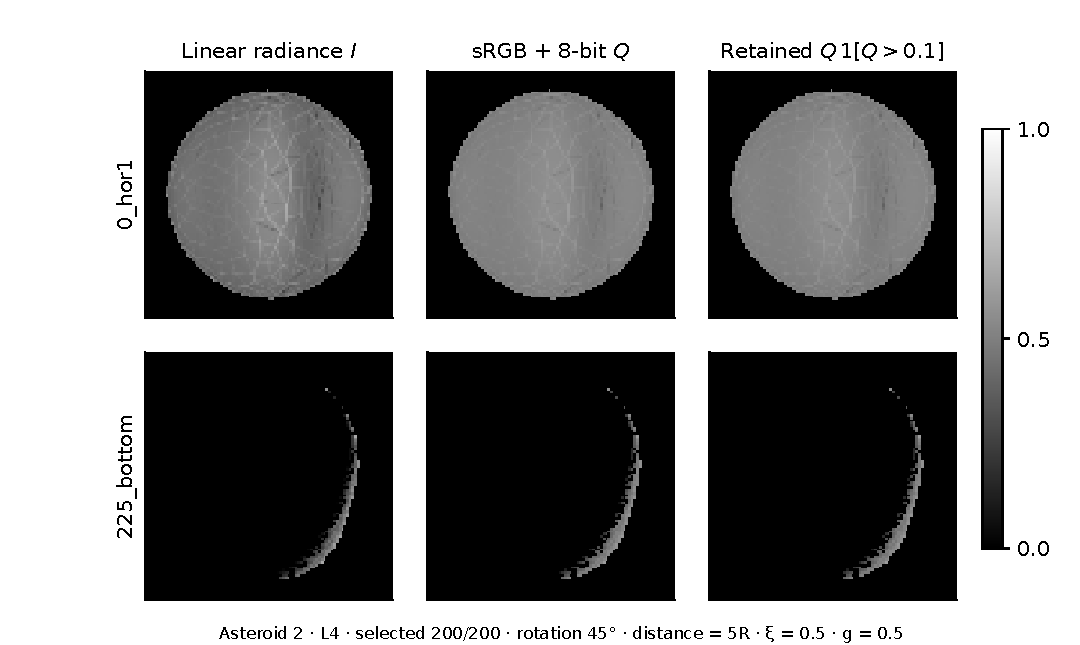
\includegraphics[width=.94\linewidth]{figures/image_formation.pdf}
\caption{Image formation on the selected asteroid-2 L4 mesh (iteration 200
of 200), rendered on CPU at rotation $45^\circ$. Each panel contains the
native $96\times96$ pixels enlarged without smoothing, on a common
0--1 gray scale. Left: linear radiance. Middle: sRGB response, gain 0.5,
and eight-bit quantization. Right: retained intensity after the $Q>0.1$
cutoff, not a binary silhouette. Perspective distance is $5R$, Lambert
fraction $\xi=0.5$, with a $96\times96$ shadow map and four fragments per
pixel. Encoding brightens weak radiance before the cutoff; the
\texttt{225\_bottom} view retains a thin illuminated region.}
\label{fig:image}
\end{figure}

\subsection{Normalization and phase partitions}
For a normalization set $\mathcal T$,
\begin{equation}
 \bar B_j=\frac{1}{|\mathcal T|}\sum_{t\in\mathcal T}B_{tj},\qquad
 \widehat y_{tj}=\frac{B_{tj}}{\max(\bar B_j,10^{-9})}.
 \label{eq:normalization}
\end{equation}
Training normalizes both predictions and targets over all training rows.
Render chunks never define separate normalization sets. Validation and
reporting first render all 360 phases, normalize once over the full turn,
and then select the scored rows. The supplied full-turn-normalized
observations are not renormalized on validation subsets.

The experiments use disjoint zero-based index sets
\begin{equation}
 \mathcal T_{\rm train}=\{0,5,\ldots,355\},\qquad
 \mathcal T_{\rm val}=\{2,7,\ldots,357\},
\end{equation}
with 72 rows each and all 21 cameras. The other 216 phases do not select
shape checkpoints. Denser phase coverage and full-turn scoring reduce
normalization bias for narrow, high-contrast lightcurve peaks.

\section{Empirical calibration}
Calibration precedes inversion and uses the public bodies. Each reference
is centered by its bounding box and scaled to $z$ half-extent one. A
1,280-face radial proxy is constructed on a subdivision-3 icosphere:
for each unit direction $\vect u_i$, intersect the ray
$r\vect u_i$, $r>0$, with the reference and retain the \emph{outermost}
intersection $r_i$. The proxy vertices are $r_i\vect u_i$ with the
icosphere's triangle connectivity. A direction with no hit invalidates
this construction. Figure~\ref{fig:proxy} compares the actual asteroid-3
reference and its proxy.

One radius per direction cannot represent multiple radial layers or
occluded inner surfaces. Finite angular sampling and interpolation across
triangles can also round narrow depressions and the waist between lobes.
The proxy is therefore a calibration approximation; it need not preserve
all reference geometry. With the proxy fixed, calibration minimizes pooled
intensity RMSE over acquisition parameters
$\vartheta=(\text{projection},d,\xi,T,g,\text{phase convention})$.

\begin{figure}[!htbp]
\centering
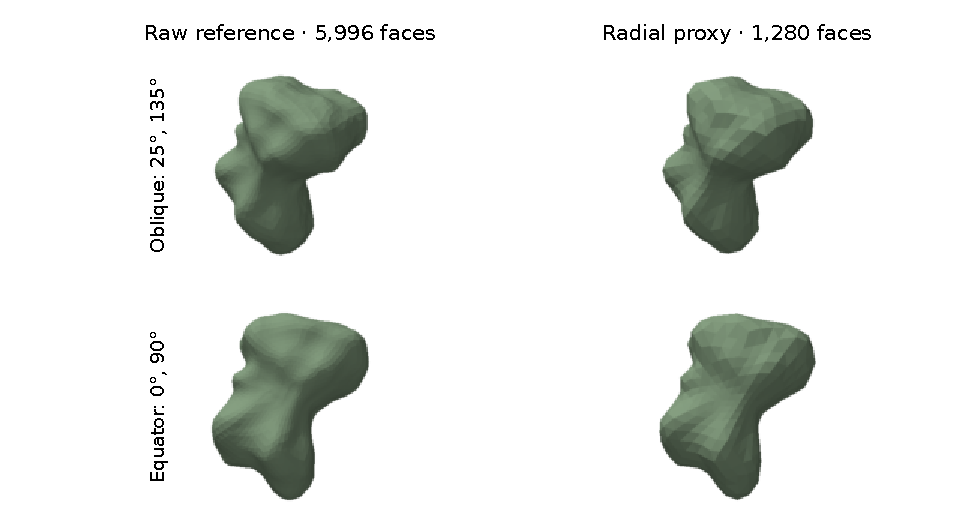
\includegraphics[width=.87\linewidth]{figures/star_proxy.pdf}
\caption{Asteroid 3: the raw 5,996-face reference and its 1,280-face radial
proxy in matched orthographic views, at the same scale and orientation.
The outermost-ray construction retains the broad two-lobed form but
changes the waist and local surface detail. Flat triangle normals and
common illustrative lighting make the tessellation visible; this is a
geometry display, not an acquisition image.}
\label{fig:proxy}
\end{figure}

The procedure screens 420 candidates per body: perspective distances
$\{2.5,3.5,5,8,16,32\}$ plus one orthographic case, mixtures
$\{0,.25,.5,.75,1\}$, two responses, gains $\{.5,1,2\}$, and two phase
conventions. Screening uses 72 phases; the top three, a baseline candidate,
and a shared-grid candidate are checked over all 360 phases. A winning
finite-distance boundary triggers one outward extension. Because linear
radiance is affine in $\xi$, Lambert and Lommel--Seeliger endpoint images
can be mixed before response and thresholding; a direct-render check
validates this acceleration.

\begin{table}[!htbp]
\centering
\caption{Public calibrations used for the L4 experiment. Scores are
full-turn pooled RMSE of calibrated public proxies, not inverse-fit errors.
All selected responses are sRGB with zero-based phase indexing.}
\begin{tabular}{@{}clrrrr@{}}
\toprule
Asteroid & Projection & $d$ & $\xi$ & $g$ & Proxy RMSE\\
\midrule
\tableinput{tables/calibration_rows.tex}
\bottomrule
\end{tabular}
\end{table}
Camera distances are effective acquisition parameters in radius units,
not measured physical intrinsics. A shared calibration increased
asteroid-2 and asteroid-3 proxy errors by 8.7\% and 47.6\% relative to
separate settings in the calibration comparison, supporting per-body
settings for public shapes.

Calibration uses public full-turn observations and shapes. Subsequent
validation scores are therefore \emph{conditional on calibration}, not
end-to-end held-out reconstruction tests. Asteroids 4--10 use asteroid 3's
calibration (orthographic projection, $\xi=0.75$, sRGB, $g=1$). This transfer
is an assumption about acquisition; their hidden references cannot verify
it or the inferred geometry.

\clearpage
\section{Regularized inverse solver}
\subsection{Objective and staged updates}
At zero-based update $k$, minimize
\begin{equation}
 \mathcal J_k(\vect p)=\frac{1}{N_{\rm train}C}
 \sum_{t,j}(\widehat y^{\rm soft}_{tj}(\vect p)-y^{\rm train}_{tj})^2
 +\lambda s_k\mathcal R(\vect p),\qquad
 \mathcal R(\vect p)=\frac{1}{146}\sum_{r=1}^{P}\ell_r^3p_r^2.
 \label{eq:loss}
\end{equation}
All samples and channels have equal weight. The denominator 146 is held
fixed across the representation comparisons, rather than averaging
over each model's own parameter count. Constants in $b,c$ have zero
spectral penalty. The prior suppresses high-degree deformation but is
not a collision or convexity constraint.

The fixed optimizer settings used for the L4 experiment are
\begin{equation}
 \lambda=1.9962845\times10^{-3},\quad
 \eta_{\rm init}=4.4673588\times10^{-3},\quad
 \eta_{\rm base}=2\times10^{-3},\quad\eta_{\min}=10^{-5}.
\end{equation}
With $T=200$ updates, $E=40$ escape updates, and $S=40$ stabilization
updates, the schedule is
\begin{equation}
 \eta_k=\begin{cases}
 \eta_{\rm base}+\dfrac{\eta_{\rm init}-\eta_{\rm base}}{2}
 [1+\cos(\pi k/(E-1))],&0\leq k<E,\\[4pt]
 \eta_{\min}+\dfrac{\eta_{\rm base}-\eta_{\min}}{2}
 [1+\cos(\pi(k-E)/(T-E-1))],&E\leq k<T.
 \end{cases}
\end{equation}
Escape masks gradients above degree two and sets $s_k=0.25$.
Refinement enables all coefficients with $s_k=1$.
During the last $S$ updates,
$s_k=1+[k-(T-S)+1]/S$, ending at twice the base prior weight.

After the degree mask, clip the gradient to Euclidean norm 10 and apply
Adam~\cite{adamoptimizer} with $(\beta_1,\beta_2)=(0.9,0.999)$ and
$\epsilon=10^{-8}$:
\begin{align}
 \vect m_k&=\beta_1\vect m_{k-1}+(1-\beta_1)\vect g_k,\qquad
 \vect v_k=\beta_2\vect v_{k-1}+(1-\beta_2)\vect g_k^{\odot2},\\
 \vect p_{k+1}&=\vect p_k-\eta_k
 \frac{\widehat{\vect m}_k}{\sqrt{\widehat{\vect v}_k}+\epsilon}.
\end{align}
Hats denote bias-corrected moments. Moments persist across stages; there
is no weight decay. Parameter projection is the identity. During fitting, finite-vertex checks detect
numerical failure; post-fit mesh audits additionally inspect degeneracy
and transverse self-intersections.

\subsection{Memory-bounded differentiation}
Training brightness depends on the mean over all training phases.
Retaining every renderer graph would be unnecessarily expensive.
The implemented two-pass scheme first renders all raw brightness in
six-frame blocks without renderer graphs, then differentiates the small
$72\times21$ brightness array. Away from the mean floor, writing
$D_{tj}=\partial\mathcal L_{\rm data}/\partial\widehat y_{tj}$ gives
\begin{equation}
 \frac{\partial\mathcal L_{\rm data}}{\partial B_{kj}}
 =\frac{D_{kj}}{\bar B_j}
 -\frac{\sum_t D_{tj}B_{tj}}{N_{\rm train}\bar B_j^2}.
 \label{eq:two-pass}
\end{equation}
Each block is then rerendered with gradients, and these brightness
derivatives are backpropagated. Add the prior once and take one optimizer
step after all blocks. This is the chain rule for the complete-set
normalization, not independent mini-batch optimization. It trades an
extra forward pass for bounded graph memory. Algebraic and CUDA checks
compare it with unchunked differentiation.

\subsection{Validation selection and reported errors}
Hard extraction evaluates the sphere and every 20 updates. The selected
state minimizes
\begin{equation}
 \RMSE_{\rm val}=\sqrt{\frac{1}{72C}
 \sum_{t\in\mathcal T_{\rm val},j}
 (\widehat y^{\rm exact}_{tj}-y_{tj})^2}.
\end{equation}
The full-turn pooled RMSE in all result tables instead uses all 360 phases
and all 21 cameras with equal weight. It is a descriptive fit error,
including both training and validation phases. Selection by validation
can therefore produce a slightly higher full-turn error than the terminal
state. The tables distinguish selected iteration from update budget.

\clearpage
\section{Experimental settings and degree comparison}
All fits use seed zero, a radius-0.5 sphere with 1,024 faces, $96\times96$
images and shadow maps, 21 cameras, the 72/72 phase split, six-frame
training blocks, fixed calibration, and the prior denominator 146.
Table~\ref{tab:budgets} distinguishes the optimization budgets.
\begin{table}[!htbp]
\centering
\caption{Experiments represented in the results. E/R/S denotes escape,
refinement, and stabilization updates; the degree comparison also applies
plateau stopping. No run is implied by a missing table entry.}
\begin{tabular}{@{}llll@{}}
\toprule
Experiment & Models & Update budget & E/R/S\\
\midrule
Ten-asteroid experiment & Octantoid L4 & 200 & 40/120/40\\
Asteroid-3 screening & Radial L6, L11; octantoid L6 & 120 & 12/96/12\\
Asteroid-1 degree comparison & Octantoid L2, L4, L6 & Cap 360 & 40/280/40$^*$\\
\bottomrule
\end{tabular}
\smallskip
\parbox{.95\linewidth}{\small $^*$Nominal schedule before stopping. After at
least 200 updates and 100 without meaningful validation improvement,
40 confirmation updates use a learning-rate ceiling reduced by factor
0.2. Improvement must exceed $\max(10^{-4},0.005\,\RMSE_{\rm reference})$.
This is a stopping rule, not a certificate of optimality.}
\label{tab:budgets}
\end{table}

\begin{table}[!htbp]
\centering
\caption{Asteroid-1 degree comparison. Scores are full-turn pooled RMSE;
stop iteration is the number of updates actually used.}
\begin{tabular}{@{}lrrrr@{}}
\toprule
Model & Selected iteration & Stop iteration & Selected RMSE & Terminal RMSE\\
\midrule
\tableinput{tables/degree_rows.tex}
\bottomrule
\end{tabular}
\label{tab:degree}
\end{table}
\begin{figure}[!htbp]
 \centering
 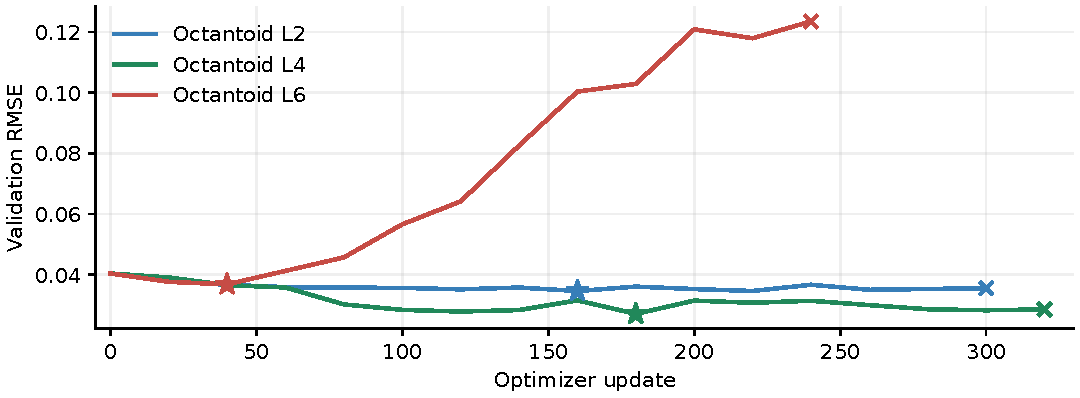
\includegraphics[width=.94\linewidth]{figures/degree_comparison.pdf}
 \caption{Exact-extraction validation histories for the asteroid-1 degree
 comparison. Stars mark selected states; crosses mark terminal states.
 Histories end at their measured stopping iterations.}
 \label{fig:convergence}
\end{figure}
L4 has the lowest selected photometric error among these three asteroid-1
fits. L6 deteriorates after its early selected state while remaining
numerically finite. The short asteroid-3 L6 fit below demonstrates that
this behavior depends on the object and optimization recipe. These
comparisons do not identify the best attainable performance of each degree
under separate tuning.

\clearpage
\section{L4 results and qualitative reconstruction}
The relative photometric improvement is
$100(\RMSE_{\rm initial}-\RMSE_{\rm selected})/\RMSE_{\rm initial}$.
\begin{table}[!htbp]
\centering
\caption{Ten-asteroid L4 experiment: identical 1,024-face sphere starts,
74 coefficients, and 200 updates per reported fit. RMSE is pooled over the
full turn and all cameras. Percentage improvement uses unrounded scores. \textemdash\ means ``no result reported.''
$\dagger$ denotes calibration transferred from asteroid 3.}
\begin{tabular}{@{}crrrr@{}}
\toprule
Asteroid & Selected iteration & Initial RMSE & Selected RMSE & Improvement\\
\midrule
\tableinput{tables/l4_rows.tex}
\bottomrule
\end{tabular}
\label{tab:l4}
\end{table}

\subsection{Asteroid 2: broad outline and residual discrepancy}
The 200-update L4 fit reduces full-turn RMSE from 0.6989 to 0.3669
(47.5\%). Figure~\ref{fig:a2} shows the selected state, not a smoothed or
reference-adjusted replacement. Its approximately square outline is
visible in the north view. Rounded edges and the absence of the raw
reference's detailed cuts remain clear in the matched views. A plausible
broad outline is weaker evidence than recovering the actual surface.

\begin{figure}[!htbp]
\centering
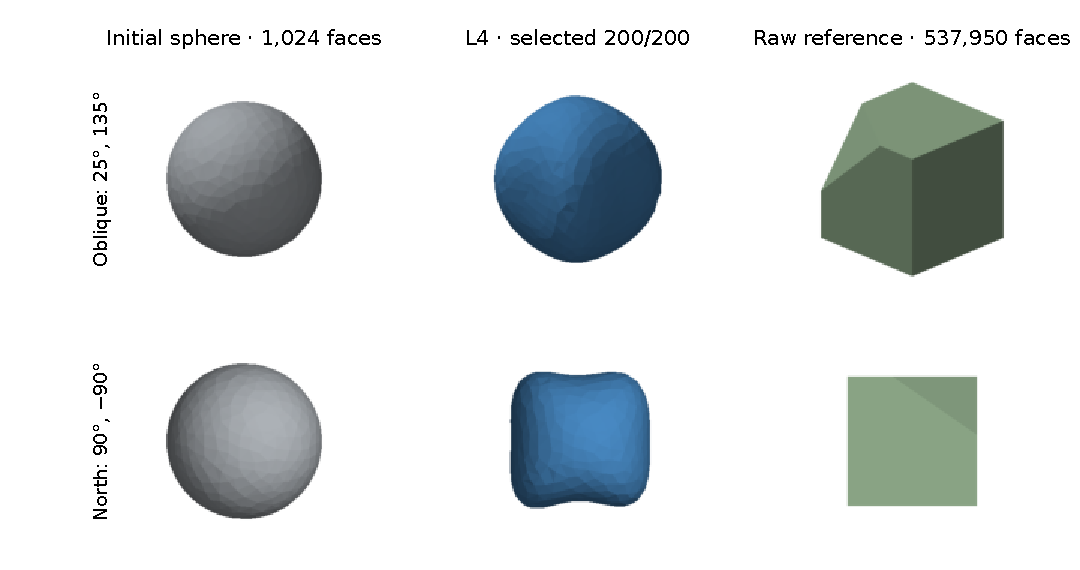
\includegraphics[width=.96\linewidth]{figures/reconstruction_asteroid2.pdf}
\caption{Asteroid 2: initial sphere, selected L4 reconstruction at iteration
200 of a 200-update fit, and the raw 537,950-face reference. Initial and
selected meshes each have 1,024 faces. Display scales are independently
aligned to the raw reference using the radial-log criterion below; no
rotation is fitted for the display. Matched camera orientation and common
framing reveal the broad square outline and the missing geometric detail.}
\label{fig:a2}
\end{figure}

\clearpage
\subsection{Asteroid 3: photometry and geometric fidelity}
The separate 120-update comparison in Table~\ref{tab:quick} uses the same
sphere and calibration across representations. The selected octantoid L6
state has the lowest photometric error, reducing the initial 0.154377 to
0.061364. It differs from asteroid 3's \emph{L4, 200-update} result in
Table~\ref{tab:l4}; these are different models and budgets.
\begin{table}[!htbp]
\centering
\caption{Asteroid-3 representation screening: 120 updates and common
calibration, mesh, and prior denominator. Scores are full-turn pooled RMSE.}
\begin{tabular}{@{}lrrrr@{}}
\toprule
Representation & Parameters & Selected iteration & Selected RMSE & Terminal RMSE\\
\midrule
\tableinput{tables/quick_rows.tex}
\bottomrule
\end{tabular}
\label{tab:quick}
\end{table}
\begin{figure}[!htbp]
\centering
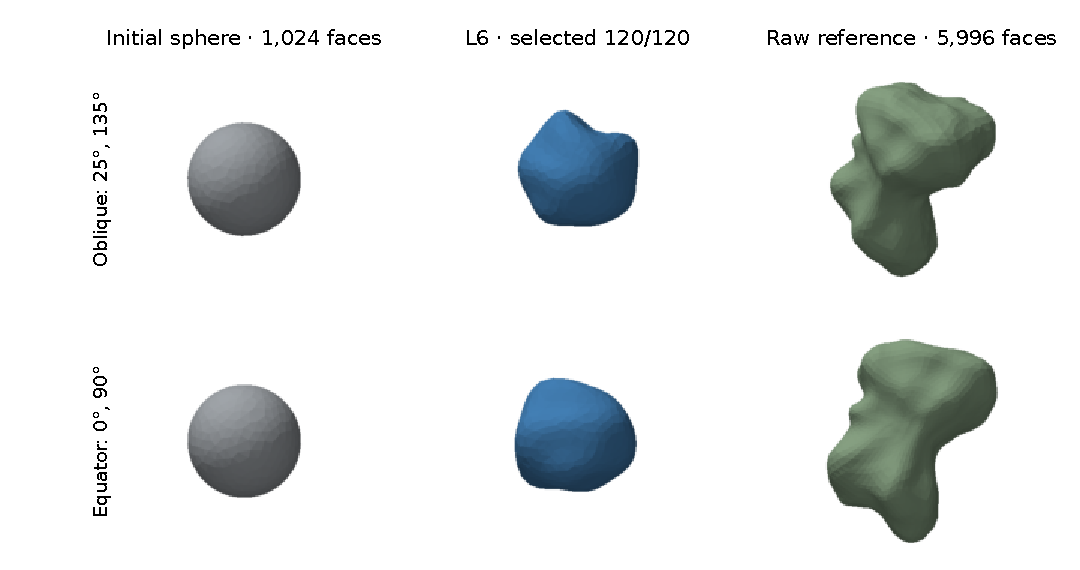
\includegraphics[width=.96\linewidth]{figures/reconstruction_asteroid3.pdf}
\caption{Asteroid 3: initial sphere, selected octantoid L6 at iteration 120
of a 120-update fit, and the raw 5,996-face reference. Matched views and
scale-only alignment expose a broad two-lobed tendency but a substantial
discrepancy in lobe proportions, neck shape, and overall extent. The
reference here is the raw surface, not the 1,280-face proxy in
Figure~\ref{fig:proxy}. The 120-update budget differs from the 200-update L4
examples for asteroids 2 and 6.}
\label{fig:a3}
\end{figure}

For public bodies, a geometry diagnostic samples 4,096 common Fibonacci
directions and compares outer radii $r_q^{\rm fit},r_q^{\rm ref}$ after
aligning a global scale only:
\begin{equation}
 \log s^*=\frac1Q\sum_q\log\frac{r_q^{\rm ref}}{r_q^{\rm fit}},\qquad
 E_{\rm geom}=\sqrt{\frac1Q\sum_q
 \left[\log\frac{s^*r_q^{\rm fit}}{r_q^{\rm ref}}\right]^2}.
\end{equation}
This measures the outer radial surface, not hidden cavities. The selected
asteroid-2 L4 geometry error is 0.1064 (initial 0.1193). For asteroid 3,
selected L6 octantoid error is 0.4930, compared with 0.4739 for radial L6,
despite the octantoid's lower photometric error. Figure~\ref{fig:a3} makes
this limitation visible. Neither the surface prior nor photometric
selection guarantees geometric accuracy.

\clearpage
\section{Asteroid 6 and interpretation limits}
Asteroid 6's selected L4 state is iteration 200 of a 200-update fit.
Its full-turn RMSE improves from 0.4598 to 0.1517 (67.0\%). The
complementary views in Figure~\ref{fig:a6} suggest a box-like form with a
crater-like depression. This is an \textbf{unverified interpretation},
conditional on the calibration transferred from asteroid 3. There is no
public reference surface for asteroid 6. Photometric agreement does not
verify the depression, its depth, or the overall geometry.
\begin{figure}[!htbp]
\centering
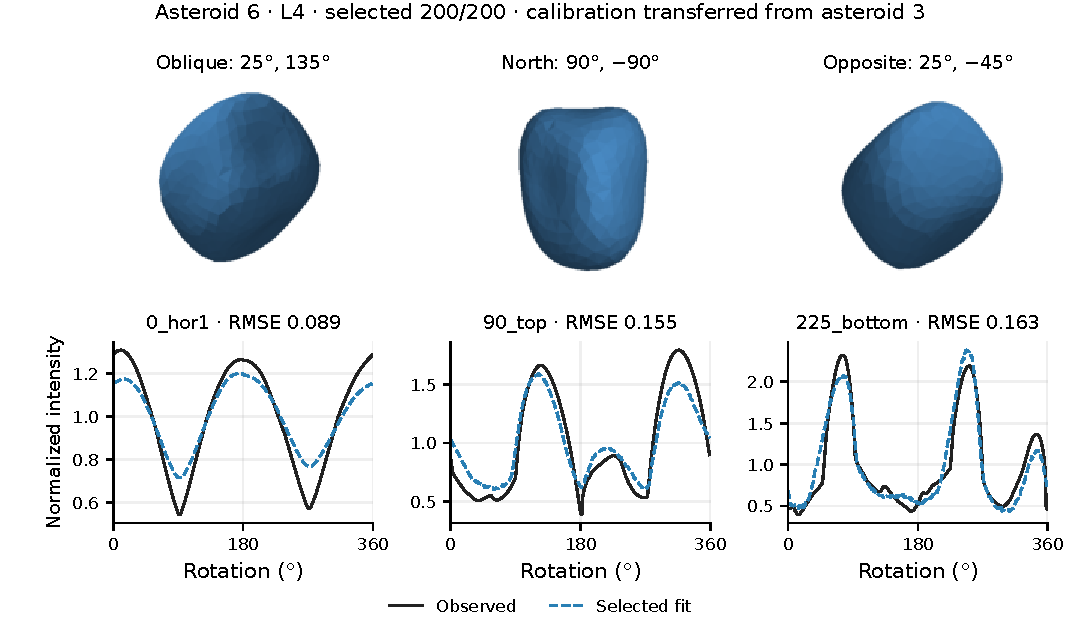
\includegraphics[width=.98\linewidth]{figures/asteroid6.pdf}
\caption{Asteroid 6: complementary geometry views of the same selected L4
mesh (200/200 updates), with observed and fitted full-turn lightcurves
for a horizontal, an upper, and a lower channel. These channels sample
different viewing geometries; the table score uses all 21. Curves are
reproduced directly from the saved selected fit. The mesh views use common
illustrative lighting and framing. A box-like form and crater-like
depression are unverified interpretations under transferred calibration.}
\label{fig:a6}
\end{figure}

Normalized photometry is non-unique: different shapes and acquisition
settings can yield similar disk-integrated curves. The finite harmonic
basis, fixed mesh connectivity, proxy calibration, approximate shadows,
and difference between soft training and hard scoring introduce further
model dependence. Fixed spherical topology excludes disconnected bodies;
positive coordinate multipliers do not exclude self-intersection. Mesh
validity audits detect numerical or geometric defects, but they cannot
establish correspondence to a hidden reference. No physical size, albedo
map, spin pole, or period is inferred by these fits.

Figures and tables reproduce saved fits without changing experiment
settings. The source bundle contains generated figures, native image
arrays, table fragments, and input hashes. Claims are restricted to the
reported measurements and budgets; missing entries supply no evidence
about fit quality or geometry.

\begingroup
\small
\setlength{\parskip}{0pt}
\begin{thebibliography}{9}
\setlength{\itemsep}{1pt}
\bibitem{octantoid}
M.~Kaasalainen and M.~Viikinkoski.
\emph{Shape reconstruction of irregular bodies with multiple complementary data sources}.
Astronomy \& Astrophysics 543, A97, 2012.
\url{https://doi.org/10.1051/0004-6361/201219267}.

\bibitem{adam}
M.~Viikinkoski, M.~Kaasalainen, and J.~\v{D}urech.
\emph{ADAM: a general method for using various data types in asteroid reconstruction}.
Astronomy \& Astrophysics 576, A8, 2015.
\url{https://doi.org/10.1051/0004-6361/201425259}.

\bibitem{lommel}
K.~Muinonen and K.~Lumme.
\emph{Disk-integrated brightness of a Lommel--Seeliger scattering ellipsoidal asteroid}.
Astronomy \& Astrophysics 584, A23, 2015.
\url{https://doi.org/10.1051/0004-6361/201526456}.

\bibitem{pytorch3d}
N.~Ravi et al.
\emph{Accelerating 3D Deep Learning with PyTorch3D}.
arXiv:2007.08501, 2020. \url{https://arxiv.org/abs/2007.08501}.

\bibitem{adamoptimizer}
D.~P. Kingma and J.~Ba.
\emph{Adam: A Method for Stochastic Optimization}.
ICLR, 2015. \url{https://arxiv.org/abs/1412.6980}.
\end{thebibliography}
\endgroup
\end{document}
